%%%%%%%%%%%%%%%%%%%%%%%%%%%%%%%%%%%%%%%%%
% University Assignment Title Page 
% LaTeX Template
% Version 1.0 (27/12/12)
%
% This template has been downloaded from:
% http://www.LaTeXTemplates.com
%
% Original author:
% WikiBooks (http://en.wikibooks.org/wiki/LaTeX/Title_Creation)
%
% License:
% CC BY-NC-SA 3.0 (http://creativecommons.org/licenses/by-nc-sa/3.0/)
% 
% Instructions for using this template:
% This title page is capable of being compiled as is. This is not useful for 
% including it in another document. To do this, you have two options: 
%
% 1) Copy/paste everything between \begin{document} and \end{document} 
% starting at \begin{titlepage} and paste this into another LaTeX file where you 
% want your title page.
% OR
% 2) Remove everything outside the \begin{titlepage} and \end{titlepage} and 
% move this file to the same directory as the LaTeX file you wish to add it to. 
% Then add \input{./title_page_1.tex} to your LaTeX file where you want your
% title page.
%
%%%%%%%%%%%%%%%%%%%%%%%%%%%%%%%%%%%%%%%%%
%\title{Title page with logo}
%----------------------------------------------------------------------------------------
%   PACKAGES AND OTHER DOCUMENT CONFIGURATIONS
%----------------------------------------------------------------------------------------

\documentclass[11pt]{article}
\usepackage[english]{babel}
\usepackage[T1]{fontenc}
\usepackage{amsmath}
\usepackage{amsfonts}
\usepackage{graphicx}
\usepackage{hyperref}
\usepackage{mathtools}
\usepackage{url}
\usepackage[colorinlistoftodos]{todonotes}
\usepackage[top=0.5 in, bottom =0.5 in, left = 0.5 in, right = 0.5 in ]{geometry}
\newcommand{\R}{\mathbb{R}}
\newcommand{\E}{\mathbb{E}}

% for bibliographic information
\usepackage{biblatex}
\bibliography{sources.bib}

% for proof environment and theorem environment (among others)
\usepackage{amsthm}

% for paragraph spacing
\setlength{\parskip}{2pt}%
\setlength{\parindent}{0pt}%

\begin{document}
\pagenumbering{roman}
\begin{titlepage}

\newcommand{\HRule}{\rule{\linewidth}{0.5mm}} % Defines a new command for the horizontal lines, change thickness here

\center % Center everything on the page
 
%----------------------------------------------------------------------------------------
%   HEADING SECTIONS
%----------------------------------------------------------------------------------------

\textsc{\LARGE Harvard University}\\[1.5cm] % Name of your university/college

%----------------------------------------------------------------------------------------
%   TITLE SECTION
%----------------------------------------------------------------------------------------

\HRule \\[0.4cm]
{ \huge \bfseries Harvard Q-Guide Predictions Market}\\[0.4cm] % Title of your document
\HRule \\[1.5cm]
 
%----------------------------------------------------------------------------------------
%   AUTHOR SECTION
%----------------------------------------------------------------------------------------

\begin{minipage}{0.4\textwidth}
\begin{flushleft} \large
\emph{Author:}\\
Luis A. \textsc{Perez} % Your name
\end{flushleft}
\end{minipage}
~
\begin{minipage}{0.4\textwidth}
\begin{flushright} \large
\emph{Author:} \\
Tiffany (Haotian) \textsc{Wu} % Supervisor's Name
\end{flushright}
\end{minipage}\\[2cm]

%----------------------------------------------------------------------------------------
%   DATE SECTION
%----------------------------------------------------------------------------------------

{\large \today}\\[2cm] % Date, change the \today to a set date if you want to be precise

%----------------------------------------------------------------------------------------
%   LOGO SECTION
%----------------------------------------------------------------------------------------


\includegraphics{logo.png}\\[1cm] % Include a department/university logo - this will require the graphicx package
 
%----------------------------------------------------------------------------------------

\vfill % Fill the rest of the page with whitespace

\end{titlepage}

\begin{abstract}
Given the announcement by Harvard College to stop publishing difficulty rating for courses \cite{crimson}, a need has arisen for alternative methods of information gathering among undergraduates. In this paper, we propose different prediction market mechanisms, detailing user input/output, contract definitions, and payment rules for each of the proposed mechanisms. The goal of each mechanism is to obtain accurate predictions that could replace Q-guide data (overall course quality, difficulty rating, and workload rating). We further discuss properties of each prediction market, such as the truthfulness incentives of for individual agents, individual agent's optimal policies, and expected results from each market. We conclude with a discussion and explanation of a simple toy implementation of the market, detailing design consideration that might affect user behaviour in our market, and laying the groundwork for future expansion and testing. 
\end{abstract}

\newpage
\tableofcontents
\listoffigures
\newpage
\pagenumbering{arabic}

\section{Introduction}
Financial markets are a well-studied area of economic theory, but with the help of the Internet, a new type of market has emerged. According to Wolfers and Zitzewitz, these new and emerging forms of financial markets, better known as prediction markets, information markets, or event futures, have the potential to collect all information about and event and thereby predict the likelihood of said event accurately \cite{wolfers}. These markets lie somewhere between large financial markets where the instruments traded are financial assets and smaller, sometimes illegal, gambling markets.  

\subsection{Prediction Markets}
Despite the question of legality, multiple prediction markets have been implemented. The markets have usually outperformed other means of information gathering, including surveys of experts. The main area of applications has thus far focused on political prediction markets, taking advantage of the win/lose binary inherent to elections to create simple to understand and simple to use open market mechanism. However, more complicated prediction markets, even for elections, have recently been proposed and tested by Dudkik et al. \cite{dudik}. Empirical results on prediction markets have demonstrated their ability to outperform other methods, especially if the markets are well-designed.

Given the effectiveness of prediction markets, they represent an intriguing solution to the problem of information gathering for undergraduate students. Specifically, students at Harvard University often optimize their class schedules using information about courses based on previous offerings. While word-of-mouth details play an important role in the student's decision-making process, a significant portion of their rational is typically based off the Harvard Q Guide \cite{cue}. 

\subsection{Q-Guide Mechanism}
The Q-guide mechanism is essentially a survey based mechanism for information gathering. As discussed by Dudik et al, this mechanism has been shown to be inferior to a prediction market in many situations \cite{dudik}. The Q-guide includes multiple additional questions for students. The questions vary from quantifiable ``workload'' to more general feedback request questions. We focus on explaining the process used for the more quantifiable axes: overall, workload, and difficulty. First, let $N$ be the set of students reporting on the Q-guide. Then the axes are:
\begin{itemize}
\item \textbf{Overall}: The scale ranges from 1.0 to 5.0. Each student is asked to given an ``overall'' rating to a course, $\hat{o}_i \in [1,5]\cap \mathbb{Z}$. As we can see, students are restricted to integer values for reporting. Once all results are in, the average is calculated and rounded to the nearest tenth. The overall score for a class is given by:
\begin{align}
\hat{o} &= \frac{1}{|N|}\sum_{i \in N}\hat{o}_i
\end{align}

where $\hat{o}$ is rounded to the nearest tenth.
\item \textbf{Workload}: The scale ranges from 1.0 to 5.0. Each student is asked to provide an integer number of ``hours spent on coursework outside of class,'' formally $\hat{w}_i \in \mathbb{N}^+$. The values are then bucketed into five distinct buckets each with unique values in the range $[1,5] \cap \mathbb{Z}$. The translation from this space of reports to the score reported in the Q-guide can be modeled by the function $f: \mathbb{N} \mapsto [1,5] \cap \mathbb{Z}$ defined as:
\begin{align}
f(\hat{w_i}) = \left\{
     \begin{array}{lr}
       1 & : \hat{w}_i \in [0, 3) \\
       2 & : \hat{w}_i \in [3, 6]  \\
       3 & :  \hat{w}_i \in [7, 10] \\
       4 & : \hat{w}_i \in [11, 14] \\
       5 & : \hat{w}_i \in [14,\infty) 
     \end{array}
   \right.
\end{align}
Given the above assignments, the result is then taken and averaged to the nearest tenth. Formally, the final workload score reported on the Q-Guide is given by $\hat{w} \in [1,5]$:
\begin{align}
\hat{w} = \frac{1}{|N|}\sum_{i \in N} f(\hat{w}_i)
\end{align}

A close look at the buckets leads rise to the following curiosity. What happens if a student reports some $\hat{r} = 3.5$, for example? Well, given the above described mechanism, this value is invalid. Contact with the college verifies our above assumptions. Only integer values are accepted in the form, and these value are then bucketed as described (possibly in an attempt to reduce the effect of outliers) and the resulting values averaged. Therefore, a report $\hat{w}_i \geq\geq 15$ is equivalent to a report $\hat{w}_i = 15$. Intuitively, it appears that this system would lead to an under-report in workload.
\item \textbf{Difficulty}: The scale once again ranges from 1.0 to 5.0. Each students $i$ is asked to report an integer number representing the ``difficulty'' of the course, $\hat{d}_i \in [1,5]  \cap \mathbb{Z}$. The result is then averaged, with final reported difficulty $\hat{d}$ of:
\begin{align}
\hat{d} &= \frac{1}{|N|}\sum_{i \in N} \hat{d}_i
\end{align}
\end{itemize}
 In general, while better than nothing, the Q-guide mechanism is imperfect. The clearest example of this is the recent decision by the administration to remove the ``difficulty'' rating from the Q-guide due to issue of subjectivity (in addition to concerns that it would lead students away from difficult but beneficial courses). 

\subsection{Benefits over Q-Guide System}
There exists some general benefits to a Harvard Q-Guide Prediction market over the current survey based mechanism. If implemented efficiently, which is discussed later in the paper, the Harvard Prediction Market can provide benefits over the Q-guide to both students and staff. First, we focus on general benefits for both staff and students:
\begin{itemize}
\item \textit{Increased influence of knowledgeable actors -} Those who have more information about the workload of a course (professors, teaching staff, etc.) would be have the incentive to influence the market more than those who are uncertain.
\item \textit{Real-time updates to scores -} With a prediction market, statistics on courses can be tracked continuously as the semester progresses. In contrast, Q-Guide Scores decrease in relevance as the year progresses. In certain years, changes to teaching staff or outside events (such as missing days from snow storms leading to significant changes in the course curriculum) could lead to a significant divergence on course data from previous years. 
\end{itemize}
 The market has several benefits for both students and teaching staff.

 Possible benefits for students:
\begin{itemize}
\item \textit{Ability to add or drop classes with accurate information -} Instead of basing decision on outdated course statistics, students can gauge aggregate class statistics before the add/drop or withdrawal deadline. It gives students a better information mechanism for decision making. 
\item \textit{Fun -} Students can compete with each other on who will ``win'' the most from the prediction market.
\end{itemize}
Possible benefits for staff:
\begin{itemize}
\item \textit{Aligning reporting incentives -} Unlike the Q-guide (where there is an incentive to complete the survey, rather than to report truthfully), a prediction market provides a selfish incentive for students to report accurately. 
\item \textit{Knowledge of how to improve the class -} With each incoming set of students, the class composition changes (prior knowledge of each set of students is slightly different). Staff can attempt to modify the course to best suit incoming classes.  However, this introduces a feedback loop issue where students might attempt to game the system. For example, they could over report the work-load in order to have the course staff modify the course itself to becomes less time intensive. 
\end{itemize}

\section{Prediction Market Mechanisms}
In this section, we explore in detail for different prediction market implementations. The goal of the prediction market will be to predict three things:
\begin{enumerate}
\item Expected Workload Rating
\item Expected Overall Rating
\item Expected Difficulty Rating
\end{enumerate}
\label{sec:examples}
 We first tackle the problem from a simplistic perspective, utilizing binary contracts as discussed in class with an automated market maker. As the paper progresses, we explore more complex extensions of the simple binary contract model, such as generalized many-contract models, and continuous-valued index-contracts. First, we tackle an important design decision which is assumed throughout the remaining models. 

\subsection{Clearing the Market}
 As with any market, an important question to resolve for the Harvard Prediction Market is the clearing mechanism that will be utilized. Current prediction markets, such as the Iowa Electronic Markets, the TradeSports market, and Foresight Exchange (to name a few) typically utilize some variation of a continuous double auction \cite{wolfers} for their trading mechanism. The benefit of a continuous double auction mechanisms lies in its simplicity. Continuous double auction markets maintain a bid-ask ledger or table for each type of contract traded. An example table is shown in Table \ref{tab:chart}.
 
 \begin{table}[h]
 \centering
    \begin{tabular}{cclll}
    \cline{1-2} \cline{5-5}
    \multicolumn{1}{|c|}{Bids (Buys)} & \multicolumn{1}{c|}{Asks}    &  & \multicolumn{1}{l|}{} & \multicolumn{1}{l|}{Trades} \\ \cline{1-2} \cline{5-5} 
    10 @ $\$3.45^*$                       & 5 @ $\$3.44^*$                     &  &                       & 5 @ $\$3.445^* $                  \\
    1 @ \$3.46                          & 1 @ \$3.45                     &  &                       & 10 @ \$3.41                            \\
    \multicolumn{1}{l}{100 @ 4.00}    & \multicolumn{1}{l}{10@ 3.45} &  &                       &                            
    \end{tabular}
    \caption{Simple example of bid-ask chart along with trade history. * marks a trade that is about to occur.}
    \label{tab:chart}
\end{table}

 At the start of the market, the ledger $\mathcal{L}$ begins empty with no bids included. A set of market participants, $N = \{1, \cdots, n\}$ then enter the market and can place buy orders, $b^{(t)}_i$, or sell orders, $s^{(t)}_i$ in sequential order. From this point forward, we use $o^{(t)}_i$ to represent either a buy or sell order. The orders can be thought of as tuples, $o^{(t)}_i = (x,p)$, where $x$ is the number of contracts the $i$-th bidder is looking to buy or sell, and $p$ is the price she's willing to pay for each contract.  When an agent $i$ places an order $o^{t}_i$ at time period $t$, for example, the order is added on the ledger $\mathcal{L}$ so that $\mathcal{L}' = \mathcal{L} \cup \{ o^{t}_i\}$. Typically, the ledger is maintained in sorted order where the buy orders are sorted in increasing order and the sell orders in decreasing order. Maintaining contra-positive sort property throughout the auction allows for efficient clearing of trades. 

Trade clearing occurs when there exists a sell order with a lower price than a buy order. More formally, let $\tilde{b}^{(t_i)}_i = (x_i,p_i) \in \mathcal{L}$ and $\tilde{s}^{(t_j)}_j = (x_j,p_j) \in \mathcal{L}$ be the buy order with the highest price (out of all buy orders $b \in \mathcal{L}$) and the sell order with the lowest price (out of all sell orders $s \in \mathcal{L}$), respectively. Then a trade occurs between $i,j \in N$ where agent $i$ sells $\min\{x_i,x_j \}$ contracts to agent $j$ at an agreed upont price $\tilde{p}$ when:
\begin{align}
p_i > p_j 
\label{eq:trade_occurs}
\end{align}
The agreed upon price $\tilde{p}$ depends on multiple factors. One possible approach is to give preference to those who have submitted an order earlier, so that $\tilde{p} = p_i$ if $t_i \leq t_j$ and $\tilde{p} = p_j$ otherwise, where we've given preference to buy orders (if submitted at the same time). However, the market can be designed so that same time submissions are impossible or made impossible by a system which arbitrarily picks one over the other, and therefore no preference is given. A second option is to simply have the agreed upon price be the median of the buyer and seller (as is the case in Table \ref{tab:chart}:
\begin{align}
\hat{p} = \frac{p_i + p_j}{2}
\end{align}
In either scenario, no trades are accepted until the transaction is settled by both parties. As we can see from the formal definition of the continuous double auction mechanism, some benefits immediately become apparent.
\begin{itemize}
\item \textbf{Continuous}: Trades occur asynchronously as soon as Equation \ref{eq:trade_occurs} is satisfied.
\item \textbf{Double}: The ledger $\mathcal{L}$ can be better thought of as two tables, $\mathcal{L} = (\mathcal{B}, \mathcal{S})$. We can do this by have that $\forall o \in \mathcal{L}$, $o = b \in \mathcal{B}$ if $o$ is a buy order and $o = s \in \mathcal{S}$ if $o$ is a sell order. We then maintain an order of $\mathcal{B}$ and $\mathcal{S}$ as previously specified. Therefore, this auction has both buyers and sellers participating disjointly, with trades occurring only between $b_i \in \mathcal{B}$ and $s_j \in \mathcal{S}$ where $\mathcal{B} \cap \mathcal{S} = \emptyset$. 
\end{itemize}

However, a secondary option for clearing the market is one which utilizes an automated market maker. While Continuous Double Auctions are simple to design and implement, the issue of liquidity quickly arises. Given that the vast majority of Harvard courses have classes of small size (average class size of below 40), it seems that this will be of particular difficulty in a Harvard Predictions Market for Q-Guide data. With this in mind, we now turn to an exploration of automatic market makers. While the system above would have provided us with a relatively simple implementation of a market, it would likely have led to low liquidity and by extension an inefficient market which would have provided little more information.

The idea of an automated market maker is to have an agent disjoint from our set $N$ of current market participants with whom all trades occur. As opposed to the CDA concept where we have trades occurring between $i,j \in N$ when the market forces dictated, with an automatic market maker, all agents $i \in N$ trade only with the market maker. The market maker is always willing to quote some sell price $p_{i,\tau}$ per contract for a query by agent $i$ of $x_i$ contracts of type $\tau$. If paid that price, then the automatic market maker transfers $x_i$ contracts of type $\tau$ to agent $i$. Similarly, the market maker is willing to quote some buy price $p_i{i,\tau}$ per contract for a query by agent $i$ of $x_i$ contracts of type $\tau$. If paid that amount, the market maker will accept that number of contracts and pay the agent $x_ip_i$. 

With the above, liquidity is not an issue in the market. Trades can always occur because the market maker is always willing to buy or sell any amount of a contract at some calculated price. We now several different options for this mechanism, explaining the benefits and drawbacks of each.

\subsection{Binary Contracts}
\subsubsection{Contract Definition:}
The Harvard Predictions Market's main goal is to predict the workload, the difficulty, and the overall score of a particular course. Let us consider some course $C \in \mathcal{C}$, the set of all Harvard Course offerings for the upcoming semester. Then we define $\hat{w}_C \in [0,168] \cap \mathbb{Z}$ as the average number of hours per week spent by all students in course $C$ during the semester. Similarly, we can defined $\hat{d}_C,\hat{o}_C \in [1,5]$ as the reported difficulty and average overall rating for the course during the semester. We can then consider a set of corresponding random variables for each quantity, $\{ w_C, d_C, o_C \}$. All of the previous quantities will be realized when the Q-Guide results are released the following semester. However, the task of prediction market is to provide information on these random quantities before their respective events occur. 

In order to do this, we design a simple binary contract for each of the above random variables. For simplicity, we begin our focus with the contract for workload, labeled $T_w$. We can define some cutoff $c$ for the number of hours worked per week and then create a binary contract which pays outs:

\[\mbox{payment} = \begin{cases}
1 &\mbox{if } \hat{w}_C > c_C\\
0 &\mbox{otherwise}
\end{cases}\]

where $\hat{w}_C$ is the realized workload in hours and $c$ a predetermined cutoff value.

We propose a market such that for each class, there is a single contract available for purchase for each of the above prediction categories, choosing $c = \bar{c}_C$ to be the mean workload (mean difficulty, mean overall score) from the previous year for the course $C$. Essentially, this contract would predict whether the workload (difficulty, overall score) from this year is greater or less than the workload (difficulty, overall score) from previous years. Intuitively, the market provides a good amount of information, diving the space of possible prediction for each quantity into two distinct regions by our choice of $c$.  

% You can get rid of this if you want. Just explaining intuition.
It's important to choose $c$ carefully, as if we determined a global $\bar{c}$, it would offer less information. Consider the difference between an advanced grad-level CS course and a standard introductory course. It's reasonable to assume that the workload of the grad course, $\hat{w}_G$, is greater than that of the introductory course $\hat{w}_U$, so choosing $c = \bar{c}$ such that 
\[ \hat{w}_U < \bar{c} < \hat{w}_G\] might not offer much additional information, if it's known with high probability that $\hat{w}_G > \bar{c}$ already. Choosing a distinct $c = \bar{c}_C$ for each class addresses this problem.

The problem detailed above is not purely hypothetical -- we can see that while the distribution of our metrics does tend to stay away from extremes, it nonetheless does vary significantly from course to course. See Figure \ref{fig:mean_median}. While popular values for each metric consist of a set of size 3, given the small support of our data, it's important to choose our value of $c$ appropriately. Data is shown for both mean and median.

\begin{figure}[h!]
\centering
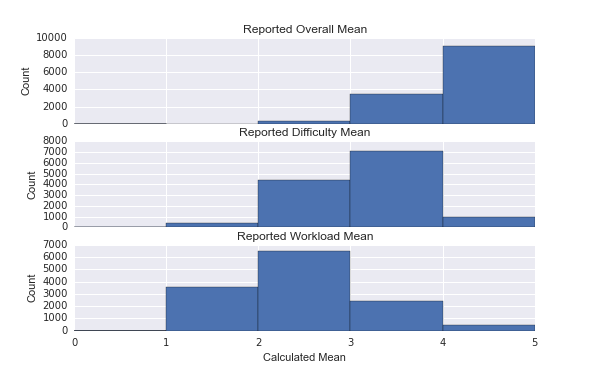
\includegraphics[scale=0.36]{mean}
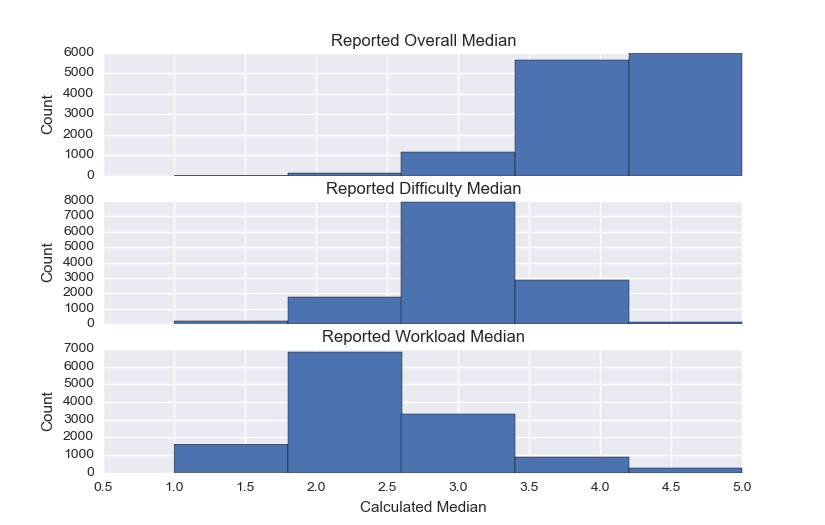
\includegraphics[scale=0.36]{median}
\caption{Histogram of Distribution for Q-Guide Data for 2014. }
\label{fig:mean_median}
\end{figure}

Another possible choice for $c$ is the median of the above each of the above statistics for each course. Given the bounded, compact, and small support for our variables, however, the mean and the median should not diverge significantly. We verify this empirically by comparing observing Figure \ref{fig:distance}. The workload metric is the one with the most variation, but even so, the difference for most courses is minor.

\begin{figure}[h!]
\centering
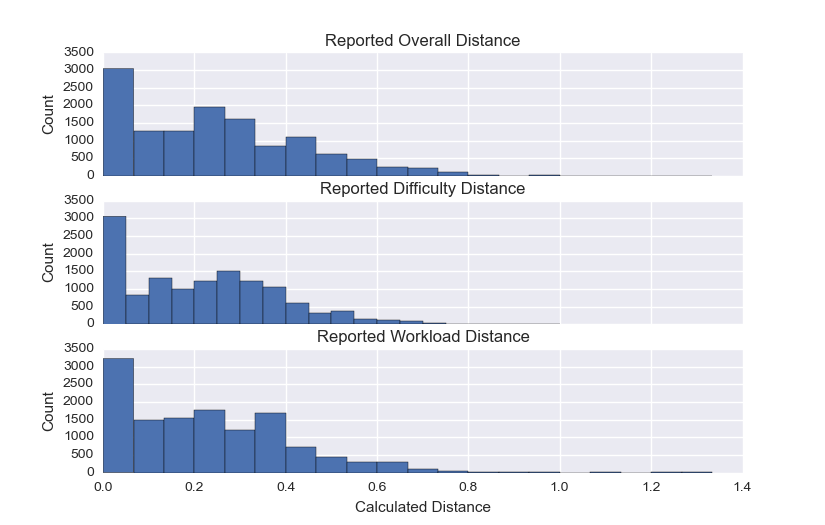
\includegraphics[scale=0.5]{distance}
\caption{Histogram of absolute distance between median and mean for Harvard Course offerings in 2014.}
\label{fig:distance}
\end{figure}

\subsubsection{Cost-based Automated Market Maker}
\label{sec:simple_maker}
We use the construction of a cost-based Automated Market Maker as defined in Parkes and Seuken's textbook. \cite{textbook} The market state is $(x_1, x_2)$, meaning that there are currently $x_1$ of contract 1 sold, and $x_2$ of contract 2 sold, where contract 1 pays out $1$ if the realized outcome $\hat{w}_C$ is greater than $c_C$, and contract 2 pays out $1$ otherwise.  

We have the cost function

\begin{equation}
C(x_1, x_2) = \beta\ln(e^{x_1/\beta}+ e^{x_2/\beta})\label{eq:costfun}
\end{equation}


where we can modify $\beta$ to adjust the sensitivity so that there are no wild price swings from any one bidder (or it is at least more difficult for the bidder to adjust the results). 

If the agent wants to shift the market state to $(x_1', x_2')$, then we charge them 

\[ C(x_1', x_2') - C(x_1, x_2)\]


The corresponding instantaneous prices are for each of the contracts $i$ are:

\begin{equation}
p_i(x_1,x_2) = \dfrac{e^{x_i/\beta}}{\sum_{j=1}^2 e^{x_{j}/\beta}}\label{eq:pricefun}
\end{equation}

\subsubsection{Desirable Properties}
As proven in Parkes and Seuken's work \cite{textbook}, the LMSR satisfies, liquidity, no arbitrage or round-trip arbitrage, myopic incentives, and bounded loss to the market maker. In our example for the Harvard Prediction market, this provides an incentive for truthfulness. Participating students would be encouraged to purchase contracts in a fashion that would cause the market to approxiamte their own belief. We can even allow for fractional purchases of contracts.

Furthermore, the cost based automated market maker defined above has the excellent property that for either contract $x_1$ or $x_2$, we have:
\begin{align}
\lim_{x_i \to \infty} C(x_1,x_2) &= \lim_{x_i \to \infty} \beta \ln (e^{x_1/\beta} + e^{x_2/\beta}) \\
&\approx \ln (e^{x_i}) \\
&\approx x_i \label{eq:linear}
\end{align}
Therefore, in order to influence the aggregate belief by a significant amount, the student would have to purchase (or sell) a significant amount of one type of contract. This near-linear relation between the strength of a belief and the cost of shifting the market to that belief gives us a market that's resilient to manipulations. We can further guarantee this by maintaining a credit system where points tend to be difficult to come by.

Furthermore, we'll have that the price paid for a set of contracts, given Equation \ref{eq:linear}, will tend to reflect the overall change in the state-space:
\begin{align}
C(x_1',x_2') - C(x_1,x_2) &\approx |x_1' + x_2' - x_1 - x_2| 
\end{align}

This model would be appropriate if we want to determine the expected difficulty rating or overall rating, where the number is more or qualitative, and the accuracy of the expected outcomes is less meaningful.

Though we could use this to determine whether or not workload has increased from last year, this might not be as much information as students or instructors desire. To do this, we can generalize this "bucketing" strategy to the continuous realm by having an infinite number of buckets, as defined in the exposition that follows.

\subsection{Generalization to Multiple-Contracts}
\label{sec:general_market_maker}
The immediate solution to the above problem is a straight-forward generalization of Equation \ref{eq:costfun}. If we want to bucket the outcomes into $n$ buckets, with thresholds $ 0< c_i \leq n$ such that $x_i$ is the number of contracts purchased that pay out $1$ point if $c_{i-1}< w \le c_{i}$. A natural division point for the Q-Data pertaining to difficulty and overall difficulty could be contracts where we have $c_i = i$ for $i \in \{0, \cdots,5\}$ (so we set $n=5$). Similarly, for the workload, we could create integer division points. This would mimick the input students already see in the Q-Guide. For Workload, we can have $n = 100$ so $c_i = i$ for $i \in \{0,\cdots,100 \}$.

We can then define a simple state vector $\vec{x} \in \R^n$ which represents the current state of the market. For a change of state to $\vec{x}'$, the cost to the students would be:
\begin{align}
C(\vec{x}') - C(\vec{x})
\end{align}
where the cost function is now a vector function $C: \R^n \to \R$:
\begin{align}
C(\vec{x}) = \beta \ln \left(\sum_{i=1}^{n} e^{\vec{x}_i}\right)
\end{align}

A ``quote'' of a price in our new system would likely serve best to quote all contract prices pertaining to a class for a given prediction metric. The reasoning behind this would be that a student could then use the values of each contract to obtain a reasonable approximation of the probability density function of the course:
\begin{align}
 	\vec\nabla_{\vec{x}} C(\vec{x}) = \left(\frac{e^{x_1/\beta}}{\sum_{i=1}^{n}e^{\vec{x}_i}}, \cdots, \frac{e^{x_n/\beta}}{\sum_{i=1}^{n}e^{\vec{x}_i}}\right)^T
\end{align}

Due to the simple generalization from the binary contract market, using an automated market maker as defined above retains the same beneficial properties discussed earlier. Now, we explore some possible drawbacks.

\subsubsection{Event Definition and Agent Response}
Note that the above bucketing strategy would pose no additional challenges in terms of defining our events -- in fact, while Q-Guide data is typically presented in a summarized fashion, the result for each reported value is released alongside. For each metric, for each class, for each contract, we would then simply payout $1$ for those contracts that fell into the correct bucket. Again, this is a straightforward generalization of the binary contract case.

It might be interesting to note, however, that contract regions are no longer evenly divided. Recall that in the binary contract, we picked the median of the values (or even the mean). Looking at the Q-Guide data from last year, as seen in Figure \ref{fig:distribution}, we note that it is incredibly unlikely for a course to receive a score in the first bucket for any of our measures. We might intuit that this would lead to some issues with the model -- however, this data is also publicly available. Students would typically be discouraged from buying contracts of type 1, unless they had information about a particular course offering no-one else did. Then it would be in their interest to purchase contracts of type 1, which assuming a distribution similar to that of previous years, would be significantly cheaper than other contracts.

\begin{figure}[h!]
\centering
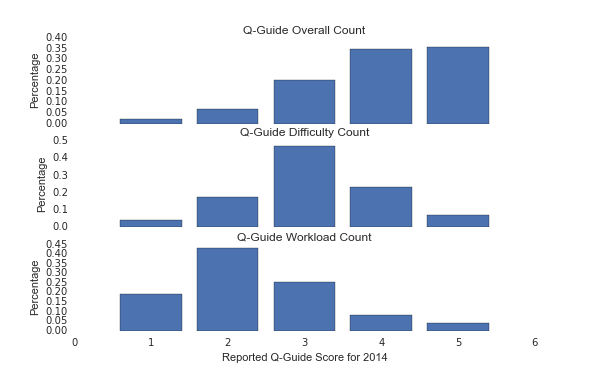
\includegraphics[scale=0.5]{distribution}
\caption{Distribution of Scores for Q-Guide 2014 Data}
\label{fig:distribution}
\end{figure}

The agent response to this change, therefore, should be minor. The difficulty would arise in the size of the number of contracts that a student buys. If we were to implement the above market solutions, we would be asking for a student to participate, on average, in the consideration for purchase of at least 60 different contracts (to cover the an expected 4 courses). No only would such a complex market likely lead to low participations (decreasing the effectiveness of our predictions), but the sheer complexity might lead to unexpected real-world results do to irrational decisions on the part of the participants (for concreteness, an example of what is meant by this is the follow: suppose dealing with some many contracts is too complicated for most people, however, they still wish to participate. Then it might be likely that most people will focus there efforts on buying only one type of contract, leading to a more extreme distribution).

A solution to this, as discussed by Parkes \cite{textbook}, is to set up a combinatorial market that allows for complex yet succinct bidding strategies. With a combinatorial market, agents can express dependence of some contracts on others, thereby minimizing the risk of irrational behavior. However, while a combinatorial market as explored by Parkes is a valid alternative, we focus on exploring another possible venue for belief reporting.

Our approach attempts to more directly models the belief distribution over each of our metrics without requiring excessive student/participant input. We lose the ability to succinctly express combinatorial dependence.


\subsection{Predicting the Distribution}
A simple approach would be to generalize the above idea. As can be seen from the data, it appears that the results are normally distributed. A few sample courses chosen at random are shown in Figure \ref{fig:random}. They corroborate the idea that the distribution of our metrics tend to follow a Gaussian distribution. Intuitively, this also makes sense in the context of a model which assumes that the reasons for a course rating are complex enough as to be modeled by a random variable per student. Then each of the reported scores in the Q-Guide $s \in \{1,\cdots,5\}$, we have a sum of random variables. 

\begin{figure}
\centering
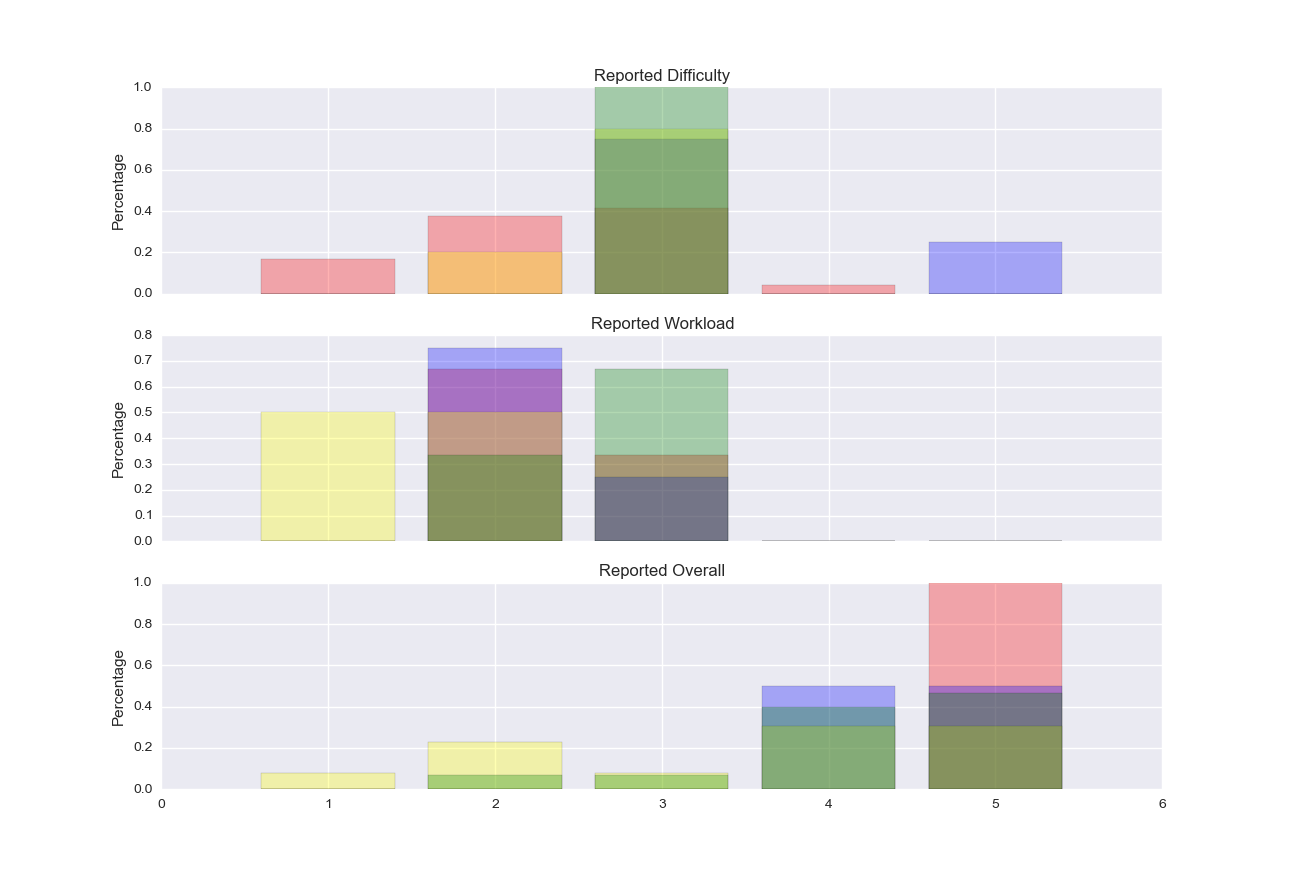
\includegraphics[scale=0.4]{random_course}
\caption{Random sampling of four course offerings at Harvard.}
\label{fig:random}
\end{figure}

As such, we can restrict our market by making a few assumption. Suppose we know the following to be the case (we drop the $C$ in an effort to be succinct):
\begin{align}
w \sim N(\mu_w,\sigma_w) \\
d \sim N(\mu_d,\sigma_d) \\
o \sim N(\mu_o,\sigma_o)
\end{align}

If we present the above data to participants, it appears safe to assume that their beliefs will also be single-peaked, and possibly distributed normally (or at least, given the data). Therefore, as opposed to relying in a market mechanism that has market participants report their belief of discrete values, we can instead as the participants to report a set of values $\{ \mu \}$ and $\{\sigma\}$ to approximate their belief \textit{distribution}. In this sense, we reduce the expected number of contracts a user has to consider down to just 24 (6 per course, 2 for each of our predictors) .In this way, we can gather a significant amount of data from the market participants with as little input as possible. 

Furthermore, if predicting the variance is considered a significant cognitive hurdle, we can use other variables. We can instead ask participants to predict $X^2$, then use the formula $\text{Var}(X) = \mathbb{E}(X^2) - \mu^2$ to calculate the variance (this is as suggested by Parkes and other \cite{textbook}, \cite{dudik}).

While this idea is good theoretically, the assumption appears rather restrictive. We therefore extend the idea further, following the literature on predicting the value continuous, real-valued variables.

\subsection{Real-valued Predictions}
When dealing with continuous outcomes, we must generalize from our simple binary or discrete case. 
To do this, we note that by reporting $q$ for a binary-valued outcome is equivalent to describing the distribution on the value of the indicator random variable $X$:
\[\Pr(X=1)= q,\,\,\,\, \Pr(X=0)= 1-q\]

We can generalize by allowing the bidders to report their believed distribution over the space $\mathcal{X}$ of possible outcomes. In our case of workload, $\mathcal{X}$ is a subset of the real line - in particular, we think it reasonable to set
\[\mathcal{X} = [0,100]\] 
as we think that the average workload of any class will not exceed 100.

Assume for the moment that reporting a distribution is easily done by the users. We shall propose a way of implementing a tool to do this reasonably efficiently later in Section \ref{sec:implementation}.

\subsubsection{Proper Scoring Rule for Distributions}
\label{sec:continuous_scoring_rule}
First, we have an exposition on scoring rules on distributions, which is more general than we need, but we think is important for the understanding of the reader. We borrow this definition of proper scoring rule on distributions from "Proper Local Scoring Rules".  \cite{distributions}

For valid state space $\mathcal{X}$, we want to determine an estimate of the distribution $Q$ over $\mathcal{X}$. Nature will determine the realized value $x\in X$, and we want to elicit user's believed distribution over the values, $P\in \mathcal{P}$, where $\mathcal{P}$ is the space of distributions over $\mathcal{X}$.

We wish to find a proper scoring rule $S: \mathcal{X}
\times \mathcal{P} \rightarrow \R$ to gauge the quality of your quote. This will be useful later when defining an Automated Market Maker with this scoring rule in Section \ref{sec:continuous_maker}. 

The expected value of $S$ is smaller the closer that $Q$ is to the actual distribution $P$, so in order to calculate payoffs in our mechanism, we must negate it, and make affine transformations later.

Before we define one, we note that for each proper scoring rule $S$, we have two components that are automatically associated with it:
\begin{align}
H(P) &\coloneqq S(P,P) \\
d(P,Q) &\coloneqq S(P,Q) - H(P)
\end{align}
$H(P)$ will turn out to be the Shannon entropy function, and $d(P,Q)$ denotes the divergence function.

This yields the following useful properties:
\begin{itemize}
\item $H(P)$ is concave in $P$.
\item $d(P,Q) - d(P,Q_0)$ is affine in $P$.
\item $d(P,Q) \ge 0$, with equality achieved at $Q=P$. 
\end{itemize}

Let $L: \mathcal{X}\times \mathcal{A}\to \R$ be a loss function, where $\mathcal{A}$ is an action space (further exposition on the action space can be found \underline{\href{http://www.ucl.ac.uk/statistics/research/pdfs/rr268.pdf}{here}})\cite{actionspaces}. 

We overload $L$ to be defined for $P\in \mathcal{P}$:
\[L(P,a) \coloneqq \mathbb{E}_{X\sim P}[L(X,a)]\]

Define the scoring rule to be
\[S(x,Q) \coloneqq L(X, a_Q)\]
where $a_Q$ is defined as $\mbox{arg}\inf_{a\in A}L(P,a)$. 

From an agent's perspective, if the agent has belief $P$, she wants to report $Q$ to minimize the scoring rule (which is the "error" of their quote $Q$) in  order to maximize their payment, $-S(x,Q)$. 

Why is $S$ strictly proper?

By definition, 
\begin{align*}
S(x,Q) &= L(x,a_Q) \rightarrow \E_P[S(x,Q)] = L(P,a_Q)\\
S(x,P) &= L(x,a_P) \rightarrow \E_P[S(x,P)] = L(P,a_P)\\
\end{align*}

Since $a_P = \mbox{arg}\inf_{a\in A}L(P,a$, we have that 
\[L(P,a_P) \le L(P,a_Q)\]
which means that the rule is proper.

The Bregman Scoring Rules \cite{distributions} is a subclass of this general class of proper scoring rules for a specific set of actions. They are of the form 

\[S(x,Q) \coloneqq \phi'\{q(x)\} + \int[\phi\{q(x)\}-q(x)\phi'\{q(x)\}]\,dx\]

with $\phi : \R^+\rightarrow \R$ concave and differentiable.

Our (generalized) familiar logarithmic scoring rule
\[S(x,Q) = -\ln(q(x))\] 
is a Bregman Scoring rule with $\phi(s) = -s\ln s$ that also happens to also be \textit{strictly} proper, the proof of which is outside the scope of this paper. 

\subsubsection{Market Scoring Rule Construction}
\label{sec:gen_scoring_rule}
How do we apply our proper scoring rule on distributions?

To define all the parameters and function definitions of Definition 18.3 of the Parkes textbook\cite{textbook} in terms of this specific application, 
we choose to use the logarithmic scoring rule $ S(x,Q) = -\ln(q(x))$, which is a specific instance of a \textit{Bregman Scoring Rule}, which is proven to be proper on pg. 4 of the Parry paper\cite{distributions}. Here, $q(x)$ is the probability density function (or probability mass function) of $x$ under distribution $Q$.

We define
\begin{align}
R(Q, x) \coloneqq -S(x,Q) &= \ln(q(x))
\end{align}
and the $i$th agent to trade \begin{itemize}
\item Receives $Q_{i-1}$ of the previous agent
\item Makes a belief report $Q_i$,
\item Receives payment $R(x,Q_i)-R(x,Q_{i-1})$ when the outcome is realized.
\end{itemize}

As before, the part of the payment dependent on $Q_{i-1}$ is fixed, so agent $i$ is trying to maximize $R(x,Q_i)$, which is a proper scoring rule over distributions.

Thus, defining the automated market maker in this way elicits an agent's true beliefs.

\subsubsection{Automated Market Maker}
\label{sec:continuous_maker}
From the literature \cite{cost-based}, its clear that there exists a strong equivalence between a proper market scoring rule and automated cost-based market makers. We now propose a cost-based market maker for our scoring rule on continuous-valued contracts as discussed in Section \ref{sec:continuous_scoring_rule}. 

The AMM we now propose is a generalization of that discussed in Section \ref{sec:general_market_maker}. Let us consider how to define the AMM for  $X \in \{o,w,d\}$ (for one of our proposed class measures). First, we let $\mathcal{S}(X) = \sigma(X)$, where $\sigma(X) = \{X \mid \Pr(X) > 0 \}$ (ie, the support of $X$).

We then define a state $s : \mathcal{S}(X) \to \R^+$ which is a function which when given a $\tau \in \mathcal{S}(X)$ (a contract of type $\tau$), we have the $s(\tau)$ is the number of contracts of type $\tau$ currently sold by the AMM. Let $\mathcal{C}$ be the space of all integrable, invertible functions whose inverse is differentiable. Then we have that $\forall s \in \mathcal{C}$, we can define the cost function $C: \mathcal{C} \to \mathbb{R}$ as:
\begin{align}
C(s) &= \beta \ln \left( \int_{\tau \in \mathcal{S}(X)} e^{\frac{s(\tau)}{\beta}} d\tau \right)
\end{align}
Furthermore, we can extend this definition for any $f \in \mathcal{C}$. Here, we can again define the sensitivity $\beta$ which is a parameter which scales the change of rate of $C(f)$ with respect to each $f(x)$. 

Additionally, we can also calculate the price of buying or selling an infinitesimal amount of contracts of type $\tau \in \mathcal{S}(X)$ using the chain rule (we abuse notation here for the sake of readibility):
\begin{align}
p_{\tau}(s) &= \frac{dC(s)}{ds(\tau)} \\
&= \frac{dC(s)}{d\tau}\cdot\frac{d\tau}{ds} \\
&=\frac{h'(s^{-1}(\tau))s'(\tau) \cdot e^{\frac{s(\tau)}{\beta}}}{\int_{x'\in\mathcal{S}(X)} e^{\frac{s(x')}{\beta}} dx'}\\
&=\frac{e^{\frac{s(\tau)}{\beta}}}{\int_{x'\in\mathcal{S}(X)} e^{\frac{s(x')}{\beta}} dx'}
\end{align}
where we have $h(\tau) = s^{-1}(\tau)$ is the inverse function of our state function. Note that this is what allows us to simplify in the last line. The simplifcation is:
\begin{align}
h'(s^{-1}(\tau))\cdot s'(\tau) &= \frac{1}{s'(s^{-1}(s^{-1}(\tau)))}\cdot s'(\tau) \\
&= \frac{1}{s'(\tau)}\cdot s'(\tau) = 1
\end{align}

The above then generates a function for the price of each of our contracts $\tau \in \mathcal{S}(X)$ which is defined as the derivative of our cost function with respect to our state function evaluated at a point $\tau$. The result is similar to that found in Equation \ref{eq:pricefun}. 

Similarly, suppose that an agent buys contracts such that the state function is changed from $s$ to $s'$. Then we charge the agent a price equivalent to:
\begin{align}
C(s') - C(s) &= \beta \ln \left(\frac{\int_{\tau \in \mathcal{S}(X)} e^{\frac{s'(\tau)}{\beta}} d\tau}{\int_{\tau \in \mathcal{S}(X)} e^{\frac{s(\tau)}{\beta}} d\tau} \right)
\end{align}

Using the proof presented in Parkes \cite{textbook} for the equivalence between the market maker presented in Section \ref{sec:simple_maker} and the logarithmic scoring rule, we now proof equivalence of our newly proposed market maker. We assume that $\beta = 1$ for simplicity. 
\begin{proof}
Consider agent $i \in N$ and the belief of event $\hat{r}$ for our continuous random variable $X$. Suppose $i$ has belief report $b_i: \mathcal{S}(X) \to [0,\infty)$ and agent $i+1$ has belief report $b_{i-1}: \mathcal{S}(X) \to [0,\infty)$ (both of these are probability density functions) where we know that $b_{i+1}(\hat{r}) > b_{i}(\hat{r})$ and the outcome corresponding to event $\hat{r}$ has occurred. Then let us define the markets initial state $s: \mathcal{S}(X) \to \R^+$ such that the following holds true:
\begin{align}
b_i(\hat{r}) &=  p_{\hat{r}}(s) = \frac{e^{s(\hat{r})}}{\int_{\tau \in \mathcal{S}(X)} e^{s(\tau)} d\tau}
\label{eq:belief}
\end{align}
That is, we must find a state $s: \mathcal{S}(X) \to \R^+$ where the above holds. We can begin with an initial agent who has uniform belief distribution. For this agent, the state would simply be given by something of the form $s(\tau) = c$ for some $c \in \mathbb{R}$. In that scenario, the instantaneous price of all the contracts is equivalent and therefore Equation \ref{eq:belief} holds.

Now we let $Q$ denote some (possibly fractional) number of contracts of type $\hat{r}$ purchased by agent $i+1$ with belief distribution $b_{i+1}$. Note that we have:
\begin{align}
b_{i+1}(\hat{r}) = p_{\hat{r}}(s') = \frac{e^{s'(\hat{r})}}{\int_{\tau \in \mathcal{S}(X)} e^{s'(\tau)} d\tau}
\end{align}
Here, we're trying to solve for $Q$ (the number of contracts agent $i+1$ should purchase to have the market match his belief). However, $Q$ has disappeared from our equation? This is not necessarily the case. Note that we simply have $Q$ hidden inside of $s': \mathcal{S}(X) \to \R^+$:
\begin{align}
   s'(\tau) &= 
   \begin{cases} 
      s(\tau) + Q & \tau = \hat{r} \\
      s(\tau) & \text{ otherwise } 
   \end{cases}
\end{align}
With this in mind, we can continue the proof. The claim is that the payment received by agent $i+1$ with belief report $b_{i+1}$ and previous agent $i$ with belief report $b_{i}$ in the market scoring rule from Section \ref{sec:gen_scoring_rule} is equivalent to the profit the trader makes with that cost-based automatic market maker once the event corresponding to $\hat{r}$ is realized. To see this, recall that the amount received int he market scoring rule when the event corresponding to $\hat{r}$ is realized is given by:
\begin{align}
\text{payment in market rule } &= \ln b_{i+1}(\hat{r}) - \ln b_{i}(\hat{r}) \\
&= \ln p_{\tau}(s') - \ln p_{\tau}(s) \\
&= \ln \left( \frac{e^{s'(\hat{r})}}{\int_{\tau \in \mathcal{S}(X)} e^{s'(\tau)} d\tau}\right) - \ln \left( \frac{e^{s(\hat{r})}}{\int_{\tau \in \mathcal{S}(X)} e^{s'(\tau)} d\tau}\right) \\
&= s'(\hat{r}) - \ln \left( \int_{\tau \in \mathcal{S}(X)} e^{s'(\tau)} d\tau\right) - s(\hat{r}) + \ln \left(\int_{\tau \in \mathcal{S}(X)} e^{s(\tau)} d\tau \right) \\
&= Q - \left[ \ln \left( \int_{\tau \in \mathcal{S}(X)} e^{s'(\tau)} d\tau\right) - \ln \left(\int_{\tau \in \mathcal{S}(X)} e^{s(\tau)} d\tau \right)  \right] \\
&= Q - [C(s') - C(s)] = \text{ profit by trader in market}
\end{align}
\end{proof}
By the above formulation, we now have an equivalence between the proposed market rule and the defined automatic market maker. All discussion in Section \ref{sec:continuous_scoring_rule} then also applies for our prediction market on continuous variables. 

However, the market maker loses an important property now that we have a continuous space $\mathcal{X}$ over which our contracts range -- the market maker no longer has bounded loss. This is to be expected, however, following the impossibility results of Gao and Chen \cite{impossible}. Therefore, the above market maker would be useful only in the event where the space becomes discreet. As a simple fix, and arbitrary threshold can be introduced at which point the market enters a state of ``panic'' and refuses to do trades. A better fix would be to have a market which plays with virtual currency, as is suggested in Section \ref{sec:implementation}. With such a market, the implications of unbounded loss becomes more manageable, in a practical sense.

\section{Proposed Implementation}
\label{sec:implementation}
In this section, we quickly present some ideas for implementation.

\subsection{User Input}
While the theory discussed in Section \ref{sec:continuous_maker} introduces an interesting example, it's difficult to image how users would input their change in state $f$. Essentially, the users will have to provide a function $u:\mathcal{S}(X) \to \mathbb{R}^+$ specifying that they wish to buy $u(\tau)$ contracts of type $\tau$. The new state $s'$ would simply become:
\[
s'(\tau) = u(\tau) + s(\tau)
\]
However, reporting a function appears rather non-trivial. This problem can be resolved by creating an excellent input mechanism. For example, as opposed to asking individuals for values, it might be of interest to see how well individuals respond to a visual input mechanism. The users could be asked to draw a graph of their probability distribution on a screen. Even more intuitively, the users could be presented with a typically graph, and then asked to move it to most closely match their belief. In our one system, it would be this distribution that is reported and taken into account when calculating the outcome payments. A sample input system is seen in Figure \ref{fig:dist}. The idea would be to have the user be able to drag the graph to their desired state.

\begin{figure}
\centering

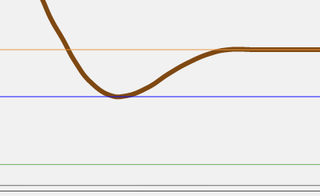
\includegraphics[scale=0.5]{dist}
\caption{Sample input mechanism}
\label{fig:dist}
\end{figure}

\subsection{Point Mechanism}
Rewards for the prediction market would also have to be thought out. Given that we cannot utilize actual money, we propose a point mechanism where individuals would gain 500 points at the beginning of each semester. They would accumulate points during their Harvard career either by remaining students (maximum of 4000), or by buying contracts and winning in different markets. In order to encourage competition, the user of the market would be ranked in a publicly accessible leader-board view-able to others, and would receive badges at different miles-stones. There would exist both a long-term leader-board, and a ``recent'' leader-board with history over only the past four years. The idea would be to have it improve competition.


\section{Conclusion}
In this paper, we focused on presenting a possible implementation of a Harvard Prediction Market. We have outlined multiple approaches to encourage truthful information collection, as well as multiple ways of avoiding potential drawbacks such as low-liquidity. Each approach balances between the effort on the part of the user and the effort on the part of the designer, as well as the trade-off between the complexity of the information gathering process and the value of the information gathered. 

The above is but a preliminary proposal on a possible implementation of the Harvard Predictions Market. More research remains to be conducted on the strategies that agents will develop as the market matures. In the immediate future, implementing the toy example discussed in Section \ref{sec:implementation} and collecting useful data would be a beneficial first step. 

On the theoretical aspect, for more information on automatic market makers for continuous random variables, we recommend the. By relaxing the restriction that each belief must be a probability density function, Chen et al. \cite{cost_based} are able to develop a general framework for bounded-loss market makers on any measurable space. The framework is likely too general for our purposes, but is nonetheless an interesting development in the field of automatic market makers. 

\printbibliography
\end{document}